\documentclass[5p,times,numbers,authoryear]{elsarticle}

\usepackage{ctex}
\usepackage{lineno}%,hyperref}
\usepackage[colorlinks,citecolor=blue]{hyperref}

\usepackage{graphics}
\usepackage{graphicx}
\usepackage{subfigure}
\usepackage{enumitem}
\usepackage{helvet}
\usepackage{courier}
\usepackage{diagbox}
\usepackage{amsmath}
\usepackage{multirow}
\usepackage{booktabs}
\usepackage{makecell}
\usepackage{amssymb}
\usepackage{threeparttable}
\usepackage[justification=centering]{caption}
\usepackage[linesnumbered,ruled,vlined,commentsnumbered]{algorithm2e}
\usepackage{color}
\usepackage{xcolor}
\usepackage{colortbl}
\usepackage{float}
\usepackage{bm}
\usepackage[normalem]{ulem} % use normalem to protect \emph
\newcommand\hl{\bgroup\markoverwith
  {\textcolor{yellow}{\rule[-.5ex]{2pt}{2.5ex}}}\ULon}

\usepackage{hyperref}
\usepackage{breakurl}

\newtheorem{definition}{Definition}
\def\boxend{\hspace*{\fill} $\Box$}
\newcommand{\comment}[1]{}
\renewcommand{\multirowsetup}{\centering}

\journal{Computers in Human Behavior}

\usepackage{appendix}

\begin{document}

\begin{frontmatter}

\title{Stress-Buffering Pattern of Positive Events on Adolescents: \\
An Exploratory Study based on Social Networks}


\begin{abstract}
Stress is viewed as the leading cause of public mental health issues.
Positive events, however, could act as a buffer against stress.
%1.�����Գ� %2.��̬�Ӿ�
Since the stress-buffering effect of positive events in previous studies was mainly examined
by subjective self-reporting,
continuous tracking research at individual behavioral levels still remains to be explored.
In this study,
We collected microblogs (n=29,232) from a high school student group (n=500) to examine the relationship
between positive events and stress-buffering pattern based on microblog content and behavioral characteristics.
%result1
Through a pilot study we found that the stress-buffering pattern of school scheduled positive events (n=259)
was manifested in both the reduction of stress intensity,
the shorter duration of stress intervals,
and talking less about academic words on micro-blog.
%result2
Hypothetical tests for stress-buffering pattern and monotonic effect of stress changes
were further conducted based on automatical extracted positive events (n=1,914) from microblogs.
The stress-buffering pattern of positive events
was closely correlated with posting behavior (ratio = 80.65\%, SD=1.96),
stress change mode (ratio = 67.74\%, SD=2.04) and microblog linguistic expressions (ratio = 74.19\%, SD=2.07).
Positive events conducted most intensive stress-buffering impact on stress from 'family life' (ratio = 83.87\%, SD=2.72),
followed by 'peer relationships' (ratio = 71.77\%, SD=4.04) and 'school life' (ratio = 67.74\%, SD=2.71) dimensions.
%restul3
Positive events buffered monotonous stress changes at both the early (11.88\% reduction) and late stages (5.88\% reduction). 
Further, the stress-buffering patterns of positive events were incorporated into the prediction of adolescents' future stress.
This study could inform the use of social network to reach and track the mental status transition of adolescents under stress.
The theoretical and practical implications, limitations of this study and future work were discussed.
\end{abstract}

\begin{keyword}
stress-buffering, positive events, microblogs, adolescents
\end{keyword}
\end{frontmatter}


\section{Introduction}
\emph{Motivation}: Life is always full of ups and downs.
Accumulated stress could drain inner resources,
leading to psychological maladjustment, depression and even suicidal behaviors \citep{Nock2008Suicide}.
Compared to adults, young people exhibit high levels of stress due to their immature inner status and lack of experience \citep{older}.
According to the latest report released by the American Psychological Association in 2018,
91\% of young adults had experienced physical or emotional symptoms due to stress in the past month compared to 74\% of adults \citep{APA2018}.
More than 30 million Chinese adolescents suffer from psychological stress,
and nearly 30\% of them are at a risk of depression \citep{ChinaTeen2019}.
Stress-induced mental health problems are becoming an important social issue. 
%1.����ѹ�����������

On the other hand, positive life events, such as satisfying social interactions,
excellent academic performance and pleasant entertainment activities, could exert protective effects on emotional distress in both direct and indirect ways by '\emph{buffering}'~\citep{Shahar2002Positive, Cohen2010Positive}, with respect to physiological, psychological, and social coping resources~\citep{Cohen1984Positive,Needles1990Positive}.
Researchers indicated that positive events mitigated the relationship between negative events and maladjustment in samples of adolescents experiencing family transitions~\citep{Doyle2003Positive}.
The written expression of positive feelings could prompt increased cognitive reorganization in undergraduate students~\citep{Coolidge2009A}.
Positive events have also been linked to medical benefits, such as improved mood, serum cortisol levels, and lower levels of inflammation and hypercoagulability~\citep{Caputo1998Influence,Jain2010Effects}.
Thus, tracking the state of the stress-buffering effect is important for understanding the mental status of stressed individuals.
%2.�����¼����Ի�������ѹ����

\emph{Existing solutions}:
Previous studies have focused on measuring positive events and stress-buffering states after events through questionnaires, including the Hassles \& Uplifts Scales~\citep{Kanner1981Comparison}, the Interpretation of Positive Events Scale~\citep{Alden2008Social},
the Adolescent Self-Rating Life Events Checklist~\citep{Jun2008Influence} and the Perceived Benefit Scales~\citep{Mcmillen1998The}.
Recently, scholars have demonstrated the feasibility to sense and predict users' stress from social networks~\citep{XueUbicomp13,Xue2014Detecting,Lin2014User,Li2015When,Li2015Predicting,Li2015Using,
Li2017Analyzing,Li2017Exploring} through content (linguistic text, emoticons and pictures) and behavioral (abnormal posting time and comment/response actions) measures.

If we view the aforementioned traditional studies as static sensing of stress-buffering, this study approaches the stress-buffering as a dynamic process and aims to find a solution at both the microblogging-content and behavioral levels under the hypothesis that the occurrence of positive events can be reflected in adolescents' microblogs.
Self-report investigations are susceptible to many factors,
such as social pressure and pressure from measurement scenarios, but microblogging characteristics at the behavioral level are objective expressions that can assist in identifying content characteristics.

Another difference from the previous studies lies in that, despite the unique advantages of social networks over traditional survey methods in offering self-expressed content and behavioral information, previous microblog-based studies stopped at the analysis of stress, and none went further to capture positive events that may play a key role in adolescents' stress-coping mechanisms.
For example, ��hiking tomorrow�� might simultaneously occur and be expressed in microblogs with ��failing the exam today��.
If do not know anything about positive events, is the unilaterally detected stress the real stressful state of the current youth?
Understanding stress-buffering patterns of positive events is helpful in precisely predicting and guiding
adolescents who are coping with stress.

\emph{Our work}:
To this end,
this paper studies adolescent stress from the dual perspective of stress generation and stress-buffering
and views stress as the superposition effect of stressors and positive events.
By investigating the connection between positive events and stress changes
reflected through adolescents' microblogging content and behaviors,
we discover stress-buffering patterns of positive events and further predict future stress under such mitigation.
Exploiting stress-buffering effects of positive events
is also advantageous in handling the confusing situation
whether an adolescent who doesn't express stressful information from microblogs is actually under stress.

However, capturing the stress-buffering process of positive events is not a trivial task.
Three fundamental challenges need to be addressed:
1) What are the criteria for depicting stress-buffering effects?
2) What is the latent connection between positive events and adolescents' stress-buffering reflections in microblogs?
3) How can identify positive events and their impact interval be extracted from microblogs?

A pilot study was first conducted on the microblog data (n=27,346) of a group of high school students (n=500) associated with the school's positive scheduled events (n=75) and stressor events (n=122).
Stressful intervals were divided into two comparative categories: intervals impacted by positive scheduled events (denoted by U-SI, n=259) and intervals not impacted by positive scheduled events (denoted by SI, n=518).
After observing the posting behaviors and microblog content of the stressed students in both the SI and U-SI groups,
several implications were discussed to guide the next step of the study.
Motivated by the implications of the pilot study, we modeled the connection between positive events and adolescents' stress-buffering reflections
as the statistical difference in two comparative situations SI and U-SI.
Three groups of measures were adopted to depict adolescent stress buffering at the period level:
stress-change modes, linguistic expressions and posting behaviors.
Monotonic changes in stress intensity buffered by positive events were measured in temporal order.
As an exploration,
according to the occurrence of automatically extracted positive events,
we covered the stress-buffering effects into each time unit and integrated such an effect into the stress prediction model.

In this paper,
to automatically extract positive events,
we built upon and extended previous stress and event detection works.
A Chinese linguistic parser model was applied to extract positive events in the linguistic structure
\emph{[type, (act, doer, description)]}.
We followed the categorization of adolescents' positive events in six dimensions (entertainment, school life, romantic, peer relationships, self-cognition and family life) and extended the SC-LIWC lexicons into 2,606 phases.
Stressful intervals (SI) and stressful intervals impacted by positive events(U-SI) were identified according to their temporal order.

The rest of the paper is organized as follows.
We review the literature in section \ref{sec:related} and introduce the pilot study in section \ref{sec:obs}.
The procedure for extracting positive events is presented in section \ref{sec:frame1}.
The connection between positive events and adolescents' stress buffering from microblogs are discussed and modeled in section \ref{sec:frame2}.
We present the experimental results in section \ref{subsec:experiment} and extend the study to integrating stress-buffering patterns into future stress prediction in section \ref{subsec:predict}.
Future work is discussed in section \ref{sec:conclude}.

\section{Literature Review}
\label{sec:related}
\subsection{Stress-buffering Function of Positive Events}
%3.����ɱ���¶��У�ѹ���ĵ�������
Positive events have been verified as protective factors against daily stress~\citep{Ong2006Psychological,Bono2013Building}, loneliness~\citep{Chang2015Loneliness}, suicide~\citep{Evan2014Social} and depression~\citep{Santos2013The}.
Through exploring naturally occurring daily stressors, \citep{Ong2006Psychological} found that over time,
the experience of positive emotions functions to assist high-resilient individuals to recover effectively from daily stress.
Through a three-week longitudinal study, \citep{Bono2013Building} examined the correlation between employee stress and health and positive life events, and concluded that naturally occurring positive events are correlated with decreased stress and improved health.
\citep{Chang2015Loneliness} investigated the protective effect of positive events in a sample of 327 adults, and found that the positive association between loneliness and psychological maladjustment was found to be weaker for those who experienced a high number of positive life events, as opposed to those who experienced a low number of positive life events.
This is assistant with the conclusion made by \citep{Evan2014Social} that positive events acted as protective factors against suicide individually and synergistically when they co-occurred,
by buffering the link between important individual differences risk variables and maladjustment.
In the survey made by \citep{Santos2013The},
strategies of positive psychology were also checked as potentially tools for the prophylaxis and treatment of depression, helping to reduce symptoms and for prevention of relapses.

%2.�����¼����õ����ַ�ʽ
The protective effect of positive events was hypothesized to operate in both directly (i.e., the more positive events people experienced, the less stress they perceived)
and indirectly ways by \emph{'buffering'} the effect of stressors ~\citep{Cohen2010Positive,Shahar2002Positive},
with respect to physiological, psychological, and social coping resources ~\citep{Cohen1984Positive, Needles1990Positive}.
%1.�����¼��������������棺�����������ۣ�������⣬�����»����¼�
\citep{Folkman2010Stress} identified three classes of coping mechanisms that were associated with positive emotion during chronic stress: positive reappraisal, problem-focused coping, and the creation of positive events.
%4. ����������¼��������ĵ�������
Due to the immature inner status and lack of experience,
adolescents exhibit more sensitive to stressors
(i.e., exams, heavy homework, isolated by classmates, family transitions),
living with frequent, long-term stress~\citep{older}.
In this situation,
positive events could help reinforce adolescents' sense of well-being~\citep{Coolidge2009A},
restore the capacity for dealing with stress~\citep{Doyle2003Positive},
and also have been linked to medical benefits, such as improving mood, serum cortisol levels, and lower levels of inflammation and hyper coagulability \citep{Jain2010Effects,Caputo1998Influence}.
The present study will be based on the consensus conclusions from the above studies.

To assess the stress-buffering effect of positive events,
scholars conducted many studies based on self-support methods.
For example,
\citep{Kanner1981Comparison} conducted Hassles \& Uplifts Scales,
and concluded that the assessment of daily hassles and uplifts might be a better approach to the prediction of adaptational outcomes than the usual life events approach.
To measure negative interpretations of positive social events,
\citep{Alden2008Social} proposed the Interpretation of Positive Events Scale, and analyzed the relationship between social interaction anxiety and the tendency to interpret positive social events in a threat-maintaining manner.
\citep{Mcmillen1998The} proposed the Perceived Benefit Scales as the new measures of self-reported positive life changes after traumatic stressors, including lifestyle changes, material gain, increases in self efficacy, family closeness, community closeness, faith in people, compassion, and spirituality.
Specific for college students,
\citep{Jun2008Influence} investigated in 282 college students using the Adolescent Self-Rating Life Events Checklist, and found that the training of positive coping style was of great benefit to improve the mental health of students.
The above explorations based on self-report investigations
were difficult to exclude interference from external factors (i.e., social appreciation, pressure from measurement scenarios).
Meanwhile, due to the lack of manpower and effective scientific methods,
most scholars relied on a limited number of measurements,
thus continuous measurements of stress-buffering process were difficult to carry out.

\subsection{Measures and Stress Analysis from Social Networks}
As billions of adolescents are recording their life through social networks (e.g., micro-blog, Twitter, Facebook),
researchers explored to apply psychological theories into social network based data mining techniques,
thus to better understand user' psychological status from the self-expressed public data source.
Multiple content and user behavioral measures have been proven effective in user mental health analysis,
including time series curve analysis of stress~\citep{Li2015When,Li2015Using}, topic words~\citep{XueUbicomp13}, abnormal posting time~\citep{Xue2014Detecting},
online shopping behaviors~\citep{DBLP:conf/apweb/Zhao0XLF16},
human mobility features~\citep{DBLP:conf/dasfaa/JinXLF16}, comment/response actions~\citep{Liang2015Teenagers}
and high dimensional multimedia features~\citep{Lin2014User}.
For example,
\citep{XueUbicomp13, Xue2014Detecting} proposed to detect adolescent stress from single post utilizing machine learning methods by extracting stressful topic words, abnormal posting time, and interactions with friends.
\citep{Lin2014User} constructed a deep neural network to combine the high-dimensional picture semantic information into stress detecting.
Based on the stress detecting result,
\citep{Li2015Predicting}\cite{Li2015Using}\cite{Li2015When} adopted a series of multi-variant time series prediction techniques (i.e., Candlestick Charts, fuzzy Candlestick line, Seasonal Autoregressive Integrated Moving Average model) to predict future stress trend.
Taking the linguistic information into consideration,
\citep{Li2017Exploring} employed a Nonlinear autoregressive with External Input Neural Network to predict a teen's future stress level referred to the impact of co-experiencing stressor events of similar companions.
\citep{Li2017Analyzing} proposed to detect stressor events from microblog content
and analyze stressful intervals based on posting rate.
All above studies focused on the discussion of stress detection on social networks.
This paper starts from a completely new perspective,
and focuses on the stress-buffering effect of positive events in adolescents' stress coping process.
Thus we push forward the study from how to find stress to the next more meaningful stage: how to cope with stress.

\subsection{Correlation Analysis Models for Multivariate Time Series}
Basic correlation analysis models on time series focused on univariate data have been well studied.
As the most widely adopted model,
the Pearson correlation analysis \cite{Cohen1988Statistical} measures the linear correlation between two variables $X$ and $Y$.
One inevitable defect of Pearson correlation is its sensitivity to outlier values.
To overcome such drawback,
Spearman Rank correlation \cite{C1987The}
and Kendall Rank correlation \cite{Mcleod2011Kendall}
were proposed based on Pearson correlation.
While Pearson correlation estimates linear relationships,
Spearman correlation estimates monotonic relationships (whether linear or not),
and are calculated as the Pearson correlation between the rank values of two variables.
The Kendall Rank correlation mainly assesses the similarity of the orderings of the data when ranked by each of the quantities.
The above correlation models are usually used to estimate relationship between single-dimensional variables,
and cannot be adopted directly in social network based scenario.

For multivariate time series analysis,
two-sample based models were widely adopted.
Such kind of models were deduced to check whether two samples come from the same underlying distribution,
which was assumed to be statistically unknown.
Correspondingly,
various kernel \citep{Sch2006A} and distance-based models \citep{Schilling1986Multivariate} were proposed.
\citep{Sch2006A} proposed to transform the distance between two variables and nearest neighbors into a reproducing kernel hilbert pace, and solve the problem using Maximum Mean Discrepancy.
\citep{Schilling1986Multivariate} adopted the $r$-nearest neighbor based model to partition two set of event driven time series data.
The global proportion of the right divided neighbors were calculated to estimate whether there existed statistically difference between the two sets.
This paper adopted the $r$-nearest neighbor based two-sample model in our problem,
thus to measure the distance and correlation between two multi-dimension variables depict
the stress-buffering patterns of positive events.

\section{Data Observation: A Pilot Study on the Stress-buffering Effect of School Scheduled Positive Events}
\paragraph{Microblogs} Microblogs of students coming from Taicang High School,
were collected from January 1st, 2012 to February 1st, 2015. 
We filtered out 124 active students according to their posting frequency from over 500 students,
and collected their microblogs throughout the whole high school career.
Totally 29,232 microblogs were collected in this research,
where 236 microblogs per student on average, 1,387 microblogs maximally and 104 posts minimally.
To protect the privacy, all usernames were anonymized during the experiment. 

\paragraph{Scheduled events} The list of weekly scheduled school events, 
with detailed description involved in the event (grade, exact start and end time), 
were collected from the school's official website\footnote{http://stg.tcedu.com.cn/col/col82722/index.html} from February 1st, 2012 to August 1st 2017.
There were 122 stressor events and 75 positive events in total. 
Examples of scheduled positive and stressor events in high school life are listed shown in Table~\ref{tab:example}.
There were 2-3 stressor events and 1-2 positive event scheduled per month in current study.
Figure~\ref{fig:example} shows three examples of a student's stress fluctuation during three mid-term exams,
where the positive event \emph{campus art festival} was scheduled ahead of the first exam (\emph{example a}),
the positive event \emph{holiday} happened after the second exam (\emph{example b}),
and no scheduled positive event was found nearby the third exam (\emph{example c}).

\begin{table}[H]
\caption{\small{Examples of school scheduled positive and stressor events.}}
\label{tab:example}
\resizebox{.45\textwidth}{9mm}{
\small{
\begin{tabular}{cccc}
\toprule
Type & Date	& Content	& Grade	\\
\midrule
stressor event & 2017/4/16 & \emph{first day of mid-term exam} & grade1,2\\
positive event & 2016/11/5 & \emph{campus art festival} & grade1,2,3\\
\bottomrule
\end{tabular}
}
}
\end{table}

\begin{figure}[H]
\centering
\includegraphics[width=\linewidth]{figs/exampleWave.eps}
\caption{\small{Examples of school scheduled positive events, stressful events, and a student's stress fluctuation}}
\label{fig:example}
\end{figure}

To further observe the effect of positive events on stressed students,
we collected all stressful intervals surround the scheduled exams over the 124 students during their high school career
applying the interval detection method in ~\citep{Li2017Analyzing}. 
For each student, we divided all stressful intervals into two sets: 
1) In the original sets, stress was caused by a stressor event, lasting for a period,
and no other intervention (namely, positive event) occured.
We called the set of such stressful intervals as \textbf{SI};
2) In the other comparative sets,
the stressful interval was impacted by a positive event(i.e., uplifts),
we called the set of such stressful intervals as \textbf{U-SI}.
Thus the difference under the two situations (sets) could be seen as the stress-buffering effect
conducted by the positive event. 
We identified 518 exam related stressful intervals (SI)
and 259 stressful intervals impacted by four typical scheduled positive events (U-SI)
('practical activity', 'new year party', 'holiday', 'sports meeting') from the students' microblogs. 
Five measures during the above two conditions were considered:
the \emph{accumulated stress}, the \emph{average stress} (per day), the \emph{length of stressful intervals},
the \emph{frequency of academic topic words}, and the \emph{ratio of academic stress among all types of stress}.
.......... 
Examples of topic words for each type of positive event were listed in table \ref{tab:keyWords}. 
Examples of academic related keywords were listed in table \ref{tab:studyWords}. 
%topic to further study
The average value of each measure over all eligible slides was calculated. 
Since our target was to track the stress-buffering effect of positive events for students under stress, 
based on previous research~\cite{XueUbicomp13}, 
we detected the stress level (ranging from 0 to 5) for each post.
For each student,
the stress value per day was aggregated by calculating the average stress of all posts. 
The positive level of each post was identified based on the frequency of positive words. 

\begin{table*}
\centering
\caption{\small{Examples of topic words for positive events.}}
\label{tab:keyWords}
\small{
\begin{tabular}{lll}
\toprule
dimension & example words & total \\ \midrule
\emph{entertainment}  & hike, travel, celebrate, dance, swimming, ticket, shopping, air ticket, theatre, party, Karaoke,& 452\\
                      & self-driving tour, game, idol, concert, movie, show, opera, baseball, running, fitness, exercise & \\
\emph{school life}    & reward, come on, progress, scholarship,admission, winner, diligent, first place, superior & 273\\
				      & hardworking, full mark,  praise, goal, courage, progress, advance, honor, collective honor& \\
\emph{romantic}       &  beloved, favor, guard, anniversary,  concern, tender, deep feeling, care, true love, promise, & 138\\
				      & cherish, kiss, embrace, dating, reluctant, honey, sweetheart, swear, love, everlasting, goddess &\\
\emph{pear relation}  & listener, company, pour out, make friends with, friendship, intimate, partner, team-mate, brotherhood& 91\\
\emph{self-cognition} & realize, achieve, applause, fight, exceed, faith, confidence, belief, positive, active, purposeful & 299\\
\emph{family life}    & harmony, filial, reunite, expecting, responsible, longevity, affable, amiability, family, duty & 184\\
\bottomrule
\end{tabular}}
\end{table*}

\begin{table}[h]
\centering
\caption{\small{Examples of academic related keywords.}}
\label{tab:studyWords}
\small{
\begin{tabular}{c}
\toprule
exam, fail, review, score, test paper, rank, pass, math, chemistry\\
homework, regress, fall behind, tension, stressed out, physics,\\
nervous, mistake, question, puzzle, difficult, lesson, careless\\
\bottomrule
\end{tabular}
}
\end{table}

\subsection{Results}
As shown in figure~\ref{fig:frequency},
comparing each measure of scheduled exam intervals under the two situations:
1) existing neighbouring positive events (U-SI) or 2) no neighbouring scheduled positive events (SI),
we found that students during exams with neighbouring positive events exhibited less average stress intensity
(78.13\% reduction in average stress, 95.58\%  reduction in cumulative stress)
and shorter duration of stress intervals (23.30\% reduction).
Further, the frequency of academic topic words (table \ref{tab:studyWords} for examples)
and the ratio of academic stress in each interval were calculated.
Results in figure~\ref{fig:frequency} shows that most students talked less about the upcoming or just-finished exams when positive events happened nearby,
with lower frequency (84.65\% reduction) and lower ratio (89.53\% reduction). 
The statistic result shows clues about the stress-buffering effect of scheduled positive events,
which is constant with the psychological theory ~\citep{Cohen1984Positive, Cohen2010Positive, Needles1990Positive},
indicating the reliability and feasibility of the microblog data set.
However,
this is an observation based on specific scheduled events,
and cannot satisfy the need for automatic, timely, and continuous perception of stress-buffering process.
Therefore, next, we will propose a framework to automatically detect positive events and its impact interval.
Based on this,
the relationship between stress-buffering effect of automatically extracted positive events and
microblog characteristics will be discussed.

\begin{figure}[h]
\centering
\includegraphics[width=0.8\linewidth]{figs/obnew-color.eps}
\caption{\small{Comparing students' stress during exam intervals in two situations:
1) intervals affected by neighboring positive events (U-SI), 2) no positive events occurred nearby (SI)}}
\label{fig:frequency}
\end{figure}

\section{Literature Review}

\section{Framework}
\subsection{Discovery of Positive Events from Microblogs}
%experiment: extraction results
\subsection{Relationship Between Positive Events and Adolescents' Stress-buffering Behaviors from Microblogs}
%��ǰ��
\subsubsection{Topic}
%�ӽ��
\subsubsection{Stress}
\subsubsection{Positive and Stressful Emotions}
\subsubsection{Posting Behaviors}
\subsection{Modeling the Stress-buffering Impact of Positive Events}
\subsection{Integrating the Stress-buffering Impact into Stress Prediction}

\section{Experiment and Evaluation}
\subsection{Setup and Metrics}
\subsection{Stress Buffering}
%KTS
%five stressors
%Measures
%pre/post
\subsection{Stress Prediction}
\section{Reference}
\bibliographystyle{model4-names}
\bibliography{reference-new}
\end{document}
